\section{Magnetismus}
Die nachfolgenden Grundlagen des Magnetismus wurden in der vierten Klausur der elften Klasse abgefragt.

\subsection{Relevante Größen und deren Zusammenhänge}

\subsubsection{Magnetische Flussdichte ($B_{\mathrm{allg}}$, $B_{\mathrm{la,\,sc}}$)}
\label{sec:magnetische_flussdichte}
Die magnetische Flussdichte $\vec{B}$ beschreibt die Stärke eines magnetischen Feldes und ist analog zur elektrischen Feldstärke $\vec{E}$ im elektrischen Feld. Sie gibt an, wie dicht die magnetischen Feldlinien in einem Bereich sind.

Wirkt eine Lorentzkraft $\vec{F}_{\mathrm{lor}}$ senkrecht auf einen Leiter, kann die magnetische Flussdichte in diesem Leiter berechnet werden:
\begin{gather}
    B_{\mathrm{allg}} = \frac{F_{\mathrm{lor}}}{I \cdot l_{\mathrm{leiter}}}
\end{gather}
\begin{center}
    \begin{tabular}{rl}
        $F_{\mathrm{lor}}$ & Lorentzkraft \\
        $I$ & Stromstärke \\
        $l_{\mathrm{leiter}}$ & Leiterlänge im Magnetfeld
    \end{tabular}
\end{center}
$B$ entspricht der Flächendichte des magnetischen Flusses $\Phi$, der senkrecht durch ein Flächenelement $A$ hindurchtritt:
\begin{gather}
    B_{\mathrm{allg}} = \frac{\Phi}{A}
\end{gather}
\begin{center}
    \begin{tabular}{rl}
        $\Phi$ & Magnetischer Fluss \\
        $A$ & Fläche
    \end{tabular}
\end{center}
In langen und schlanken Spulen (d.\,h. Länge $l$ deutlich größer als Durchmesser) gilt:
\begin{gather}
    B_{\mathrm{la,\,sc}} = \mu_0 \cdot \mu_r \cdot \frac{N \cdot I}{l}
\end{gather}
\begin{center}
    \begin{tabular}{rl}
        $N$ & Windungszahl der Spule \\
        $l$ & Länge der Spule \\
        $\mu_r$ & relative Permeabilität des Materials \\
        $\mu_0$ & magnetische Feldkonstante (aus WTR)
    \end{tabular}
\end{center}
Damit lässt sich auch der magnetische Fluss in langen und schlanken Spulen berechnen.

Die Einheit der magnetischen Flussdichte ist
\begin{center}
    $[B] = \si{\tesla} = \mathrm{Tesla} = \si{\newton\per\ampere\per\meter}$
\end{center}

\subsubsection{Magnetischer Fluss ($\Phi$)}
\label{sec:magnetischer_fluss}
Der magnetische Fluss $\Phi$ beschreibt die Menge des Magnetfeldes, die eine bestimmte Fläche durchsetzt. Er hängt sowohl von der Größe der Fläche als auch von der Orientierung des Feldes gegenüber der Fläche ab.

Die Fläche wird durch den Vektor $\vec{A}$ dargestellt, dessen Richtung der Flächennormale entspricht. Seine Länge entspricht der Größe der Fläche. Der Winkel $\theta$ gibt an, wie schräg das Magnetfeld $\vec{B}$ auf die Fläche trifft. Nur die senkrecht zur Fläche verlaufende Komponente des Feldes trägt zum Fluss bei.
\begin{gather}
    \Phi = A_{\perp} \cdot B \cdot \cos(\theta)
\end{gather}
In der vektoriellen Schreibweise wird dies kompakt durch das Skalarprodukt dargestellt. Diese Form ist besonders nützlich, wenn die Orientierung von Fläche und Magnetfeld nicht einfach geometrisch beschrieben werden kann:
\begin{gather}
    \Phi = \vec{A} \cdot \vec{B}
\end{gather}
Die Einheit des magnetischen Flusses ist
\begin{center}
    $[\Phi] = \si{\weber} = \mathrm{Weber} = \si{\tesla\meter\squared} = \si{\volt\second}$
\end{center}

\subsubsection{Lorentzkraft ($\vec{F}_{\mathrm{lor,\,leiter}}$, $\vec{F}_{\mathrm{lor,\,frei}}$)}
\label{sec:lorentzkraft}
Die Lorentzkraft $\vec{F}_{\mathrm{lor}}$ beschreibt die Kraft, die auf einen stromdurchflossenen Leiter oder auf frei bewegliche Ladungen in einem Magnetfeld wirkt. Sie entsteht durch die Wechselwirkung zwischen dem elektrischen Strom beziehungsweise den bewegten Ladungen und dem Magnetfeld $\vec{B}$.

Für einen Leiter mit Strom $I$ wirkt die Kraft auf den Abschnitt der Länge $l_{\mathrm{leiter}}$, der senkrecht zur Richtung des Magnetfeldes steht:
\begin{gather}
    \vec{F}_{\mathrm{lor,\,leiter}} = I \cdot l_{\mathrm{leiter}} \cdot \vec{B}
\end{gather}
Für einzelne freie Ladungen kann die Lorentzkraft aus der Stromformel abgeleitet werden. Mit $I = \frac{\Delta Q}{\Delta t}$ und $\frac{\Delta l}{\Delta t} = v$ folgt:
\begin{align}
    \vec{F}_{\mathrm{lor,\,frei}} &= I \, l_{\mathrm{leiter}} \, \vec{B} \nonumber \\
    &= \frac{\Delta Q}{\Delta t} \, l_{\mathrm{leiter}} \, \vec{B} \nonumber \\
    &= Q \, \frac{\Delta l}{\Delta t} \, \vec{B} \nonumber \\
    \vec{F}_{\mathrm{lor,\,frei}} &= Q \, \vec{v} \times \vec{B} \Rightarrow Q \cdot v \cdot B
\end{align}
\begin{center}
    \begin{tabular}{rl}
        $\vec{v}$ & Geschwindigkeit der Ladung $Q$ (z.\,B. eines Elektrons) \\
        $Q$ & Ladung (z.\,B. Ladung eines Elektrons  $-e$) \\
        $\vec{B}$ & Magnetische Flussdichte
    \end{tabular}
\end{center}
Das Kreuzprodukt \enquote{$\times$} zeigt an, dass die Lorentzkraft immer senkrecht zu Bewegungsrichtung und Magnetfeld wirkt. Ohne das Kreuzprodukt gilt die Formel nur für Ladungen, die sich senkrecht zum Magnetfeld bewegen.

\subsubsection{Induktivität ($L$)}
\label{sec:induktivität}
Die Induktivität $L$ ist eine physikalische Größe, die angibt, wie stark eine Spule oder ein Leiterstromkreis eine Änderung des Stromes durch die Induktion einer Spannung behindert. Sie hängt von der Geometrie der Spule, der Anzahl der Windungen und dem verwendeten Kernmaterial ab.

Die Induktivität $L$ ist definiert als das Verhältnis zwischen dem magnetischen Fluss $\Phi$ und dem Strom $I$:
\begin{gather}
    L = N \cdot \frac{\Phi}{I}
\end{gather}
Für eine lange, schlanke Spule der Länge $l$, Querschnittsfläche $A$ und $N$ Windungen im Medium mit Permeabilität $\mu_0 \mu_r$ ergibt sich:
\begin{gather}
    L = \mu_0 \mu_r \cdot \frac{N^2 \cdot A}{l}
\end{gather}
Bei der Selbstinduktion gilt für den Einschaltvorgang mit $I(0) = 0$:
\begin{align}
    U(t) &= U_0 + U_{\mathrm{ind}}(t) \\
    &= U_\mathrm{netz} - L \cdot \dot{I}(t) \\
    R_\mathrm{sp} \cdot I(t) &= U_\mathrm{netz} - L \cdot \dot{I}(t) \\
    L &= \frac{U_\mathrm{netz} - R_\mathrm{sp} \cdot I(0)}{\dot{I}(0)} \\
    &= \frac{U_\mathrm{netz}}{\dot{I}(0)}
\end{align}
\begin{center}
    \begin{tabular}{rl}
        $U_\mathrm{netz}$ & Netzspannung (Quellspannung) \\
        $R_\mathrm{sp}$ & Spulenwiderstand \\
        $\dot{I}(0)$ & Stromanstiegsgeschwindigkeit zum Zeitpunkt $t=0$
    \end{tabular}
\end{center}
$\dot{I(0)}$ ist die Anfangsänderung des Stromes, also die Steigung der Strom-Zeit-Kurve zum Zeitpunkt $t = 0$, was z.\,B. an einem Graphen abgelesen werden kann.

Die Einheit der Induktivität ist
\begin{center}
    $[L] = \si{\henry} = \mathrm{Henry} = \si{\volt\second\per\ampere}$
\end{center}

\subsubsection{Induktionsspannung ($U_{\mathrm{ind}}$)}
\label{sec:induktionsspannung}
Die Induktionsspannung $U_{\mathrm{ind}}$ ist die Spannung, die in einer Spule oder Leiterschleife entsteht, wenn sich der durch sie hindurchtretende magnetische Fluss $\Phi$ ändert. Sie ist ein direktes Ergebnis des Faraday’schen Induktionsgesetzes.

Für eine Spule mit $N_{\mathrm{ind}}$ Windungen gilt allgemein:
\begin{align}
    U_{\mathrm{ind}} &= - N_{\mathrm{ind}} \cdot \left( \frac{\Phi(t_2) - \Phi(t_1)}{t_2 - t_1} \right) \nonumber \\
                     &= - N_{\mathrm{ind}} \cdot \frac{d\Phi}{dt} \\
                     &= - N_{\mathrm{ind}} \cdot \dot{\Phi}(t)
\end{align}
Bleiben entweder die durchsetzte Fläche $A_{\perp}$ oder die magnetische Flussdichte $B$ konstant, ergeben sich vereinfachte Einzelformen:
\begin{align}
    U_{\mathrm{ind,\,konst.\,}A_{\perp}} &= - N_{\mathrm{ind}} \cdot A_{\perp} \cdot \frac{\Delta B}{\Delta t} \\
    U_{\mathrm{ind,\,konst.\,}B} &= - N_{\mathrm{ind}} \cdot B \cdot \frac{\Delta A_{\perp}}{\Delta t}
\end{align}
Unter der Annahme, dass sowohl $B(t)$ als auch $A_{\perp}(t)$ zeitabhängig sind, kann die zusammengesetzte Form über die Produktregel dargestellt werden:
\begin{gather}
    \Phi(t) = B(t) \cdot A_{\perp}(t) \\
    U_{\mathrm{ind}}(t) = - N_{\mathrm{ind}} \cdot \frac{d\Phi}{dt} \\
    \frac{d\Phi}{dt} = A_{\perp}(t) \cdot \frac{dB}{dt} + B(t) \cdot \frac{dA_{\perp}}{dt} \\
    \Rightarrow U_{\mathrm{ind}}(t) = - N_{\mathrm{ind}} \left( A_{\perp}(t) \cdot \frac{dB}{dt} + B(t) \cdot \frac{dA_{\perp}}{dt} \right) \\
    U_{\mathrm{ind}}(t) = U_{\mathrm{ind,\,konst.\,}A_{\perp}}(t) + U_{\mathrm{ind,\,konst.\,}B}(t)
\end{gather}
Bei der \hyperref[sec:bewegungsinduktion]{Bewegungsinduktion} ändert sich die durchsetzte Fläche $A_{\perp}$ durch die Bewegung eines Leiters (oft $N = 1$) im Magnetfeld. In diesem Fall wird die Induktionsspannung durch die Änderung der Fläche in Abhängigkeit der Geschwindigkeitbestimmt:
\begin{equation*}
    U_{\mathrm{ind,\,bew}} = -B \cdot \frac{dA}{dt} = -B \cdot \frac{d(x \cdot l)}{dt} = - B \cdot l \cdot \frac{dx}{dt} = - B \cdot l \cdot v_{\perp}
\end{equation*}
Bei der \hyperref[sec:selbstinduktion]{Selbstinduktion} wird die Induktionsspannung durch die Änderung des eigenen Stromes in der Spule verursacht. In diesem Fall gilt eine spezielle Form des Induktionsgesetzes:
\begin{align}
    U_{\mathrm{ind}} &= - N \cdot \frac{{d\Phi }}{{dt}} \nonumber \\
                     &= - N \cdot A \cdot \frac{{dB}}{{dt}} \nonumber \\
                     &= - N \cdot A \cdot \frac{{d\left( {{\mu _0} \mu_r \cdot \frac{N}{l} \cdot I} \right)}}{{dt}} \nonumber \\
                     &= - N \cdot A \cdot {\mu _0} \mu_r \cdot \frac{N}{l} \cdot \frac{{dI}}{{dt}} \nonumber \\
                     &= - {\mu _0} \mu_r  \cdot \frac{{A \cdot {N^2}}}{l} \cdot \frac{{dI}}{{dt}} \nonumber \\
    U_{\mathrm{ind,\,sel}} &= - L \cdot \frac{dI}{dt} = - L \cdot \dot{I}
\end{align}

\subsubsection{Energie im Magnetfeld ($W_{\mathrm{mag}}$)}
\label{sec:energie_im_magnetfeld}
In einem Magnetfeld kann Energie gespeichert werden, ähnlich wie in einem elektrischen Feld. Besonders deutlich wird dies bei einer stromdurchflossenen Spule, die ein Magnetfeld aufbaut. Der Stromfluss muss Arbeit gegen die induzierte Gegenspannung verrichten, wodurch Energie im Magnetfeld gespeichert wird.

Die gespeicherte magnetische Energie in einer Spule mit Induktivität $L$ und Strom $I$ ergibt sich zu:
\begin{gather}
    W_{\mathrm{mag}} = \frac{1}{2} \, L \, I^2
\end{gather}
Der Strom wächst an. Dabei verrichtet die Spannungsquelle Arbeit gegen die Selbstinduktionsspannung. Diese Arbeit wird in Form von magnetischer Energie im Feld gespeichert. Solange der Strom konstant ist, bleibt die Energie im Feld selbst gespeichert. Beim Ausschalten, also beim Abbau des Stroms, wird die gespeicherte Energie wieder frei, entweder geht sie wieder an den Stromkreis und wirkt dem Abbau des Stroms entgegen oder sie wird durch Widerstände in Wärme umgesetzt. Die Formel gilt immer dann, wenn sich durch eine Spule mit Induktivität $L$ bereits ein stationärer Strom $I$ eingestellt hat oder der momentane Wert $I(t)$ bekannt ist.

\subsection{Wichtige Konzepte und Vertiefung}

\subsubsection{Magnet}
\label{sec:magnet}
Ein Magnet ist ein Körper, der ein Magnetfeld erzeugt und dadurch bestimmte Materialien wie Eisen, Nickel oder Kobalt anziehen kann. Jeder Magnet besitzt stets zwei Pole, den Nordpol und den Südpol. Gleichnamige Pole stoßen einander ab, während ungleichnamige sich anziehen. Man unterscheidet zwischen Dauermagneten, die ein permanentes Magnetfeld besitzen, und Elektromagneten, deren Magnetwirkung nur während des Stromflusses auftritt.

\subsubsection{Magnetfeld}
\label{sec:magnetfeld}
Ein Magnetfeld ist der Raum um einen Magneten, in dem magnetische Kräfte wirken. Es wird durch Feldlinien dargestellt, die stets vom Nordpol zum Südpol verlaufen. Die Dichte der Feldlinien zeigt die Feldstärke an: Je dichter die Linien, desto stärker das Magnetfeld.
Ein Magnetfeld übt auf bewegte geladene Teilchen eine Kraft aus, die als Lorentzkraft $F_{\mathrm{lor}}$ bezeichnet wird. Die Richtung des Feldes lässt sich beispielsweise mit Eisenfeilspänen oder einer Kompassnadel sichtbar machen.

\subsubsection{Induktion}
\label{sec:induktion}
Ändert sich ein Magnetfeld oder die magnetische Flussdichte $\vec{B}$ in einer Leiterschleife, so wird eine Induktionsspannung $U_{\mathrm{ind}}$ erzeugt. Dies ist die Grundlage des Faraday'schen Induktionsgesetzes.
Eine Induktionsspannung tritt immer dann auf, wenn sich eine der Größen ändert, die den magnetischen Fluss $\Phi$ durch die Leiterschleife bestimmen:
\begin{itemize}
    \item die magnetische Flussdichte $\vec{B}$ des Feldes,
    \item die von der Leiterschleife eingeschlossene Fläche $A$,
    \item und theoretisch auch der Winkel $\varphi$ zwischen der Flächennormalen der Leiterschleife und der Richtung des Magnetfeldes.
\end{itemize}
Der magnetische Fluss durch eine Leiterschleife im rechten Winkel zum Magnetfeld ist gegeben durch
\begin{gather}
    \Phi = \vec{B} \cdot \vec{A} = B \, A,
\end{gather}
wobei sich eine Änderung einer der drei Größen direkt in einer Induktionsspannung widerspiegelt:
\begin{gather}
    U_{\mathrm{ind}} = - N_{\mathrm{ind}} \frac{d\Phi}{dt}.
\end{gather}

\subsubsection{Bewegungsinduktion ($U_{\mathrm{ind,\,bew}}$)}
\label{sec:bewegungsinduktion}
Bewegungsinduktion ist die Erzeugung einer Induktionsspannung $U_{\mathrm{ind,\,bew}}$, wenn ein Leiter sich relativ zu einem Magnetfeld bewegt, sodass sich der magnetische Fluss durch den Leiter ändert.
Bei einem Leiter, der auf zwei Leiterschienen orthogonal durch ein konstantes Magnetfeld gleitet, scheint sich zunächst keine der für die Induktion relevanten Größen verändert zu werden. Dennoch ist eine Induktionsspannung $U_{\mathrm{ind,\,bew}}$ messbar. Während $B$ konstant bleibt, verändert sich hier die wirksame Fläche $A$. Dies liegt daran, dass sich durch die Bewegung des Leiter der vom diesem Leiter und den Schienen umschlossene Flussbereich ändert.

In diesem Fall ändert sich $A$ mit der Zeit. Nach dem Induktionsgesetz mit $N_{\mathrm{ind}} = 1$:
\begin{equation*}
    U_{\mathrm{ind}} = -\frac{d\Phi}{dt} = -\frac{d(B \cdot A)}{dt}
\end{equation*}
Da B konstant ist, folgt für eine rechteckige Fläche der Größe $l_{\mathrm{konstant}} \cdot x$, die vom Magnetfeld durchsetzt wird:
\begin{equation*}
    U_{\mathrm{ind,\,bew}} = -B \cdot \frac{dA}{dt} = -B \cdot \frac{d(x \cdot l)}{dt} = - B \cdot l \cdot \frac{dx}{dt} = - B \cdot l \cdot v_{\perp}
\end{equation*}
Das gleiche Ergebnis lässt sich anschaulich über die Lorentzkraft nach dem Prinzip des Halleffekts nachvollziehen. Die durch den Stab in eine Richtung mitgenommenen Elektronen erfahren eine Lorentzkraft $F_{\mathrm{lor}}$, wodurch eine Ladungstrennung und damit die Spannung $U_{\mathrm{ind}}$ entsteht. Dies geschieht so lange bis $F_{\mathrm{el}} = F_{\mathrm{lor}}$. Dann gilt folgendes:
\begin{equation}
    U_{\mathrm{ind,\,bew}} = B \cdot v \cdot l
\end{equation}

\subsubsection{Selbstinduktion ($U_{\mathrm{ind,\,sel}}$)}
\label{sec:selbstinduktion}
Selbstinduktion beschreibt den Effekt, dass in einer Spule durch eine zeitliche Änderung des eigenen Stromes eine Induktionsspannung entsteht, die der Ursache der Stromänderung entgegenwirkt (Lenz'sche Regel).

Ändert sich der Strom $I(t)$ auf den Wert $I_0$ in einer Spule mit der Windungszahl $N$ und Induktivität $L$, ändert sich der magnetische Fluss und in der Spule selbst wird eine Spannung induziert. Der Strom geht nicht sofort auf seinen stationären Endwert ${I_0} = \frac{U_0}{R}$, sondern steigt allmählich auf diesen Endwert an. Das liegt daran, dass $I(t) = \frac{U(t)}{R} = \frac{U_0 - U_{\mathrm{ind,\,sel}}(t)}{R}$ gilt. Die Induktionsspannung lässt sich aus dem Induktionsgesetz herleiten:
\begin{align}
    U_{\mathrm{ind}} &= - N \cdot \frac{{d\Phi }}{{dt}} \nonumber \\
                     &= - N \cdot A \cdot \frac{{dB}}{{dt}} \nonumber \\
                     &= - N \cdot A \cdot \frac{{d\left( {{\mu _0} \mu_r \cdot \frac{N}{l} \cdot I} \right)}}{{dt}} \nonumber \\
                     &= - N \cdot A \cdot {\mu _0} \mu_r \cdot \frac{N}{l} \cdot \frac{{dI}}{{dt}} \nonumber \\
                     &= - {\mu _0} \mu_r  \cdot \frac{{A \cdot {N^2}}}{l} \cdot \frac{{dI}}{{dt}} \nonumber \\
    U_{\mathrm{ind,\,sel}} &= - L \cdot \frac{dI}{dt}
\end{align}
\begin{center}
    \begin{tabular}{rl}
        $A$ & Querschnittsfläche der Spule \\
        $l$ & Länge der Spule \\
        $\mu_0$ & magnetische Feldkonstante (aus WTR) \\
        $\mu_r$ & relative Permeabilität des Materials \\
        $N$ & Windungszahl der Spule \\
        $L$ & Induktivität der Spule \\
        $I$ & Aktueller Strom durch die Spule
    \end{tabular}
\end{center}
Diese Spannung wirkt der Stromänderung entgegen und begrenzt somit die Geschwindigkeit, mit der sich der Strom aufbaut oder abbaut.

Die Induktivität $L$ hängt von der Geometrie der Spule, der Windungszahl $N$ und dem magnetischen Kernmaterial ab. Je größer $L$, desto stärker wirkt die Selbstinduktion.
Ein typisches Beispiel ist der Einschaltvorgang einer Spule in einem Gleichstromkreis: Beim Einschalten steigt der Strom nicht sofort auf seinen Maximalwert, sondern exponentiell, da die Spule eine Gegeninduktionsspannung erzeugt. Beim Ausschalten wirkt die gleiche Spannung in entgegengesetzter Richtung.

 Siehe auch: \url{https://www.leifiphysik.de/elektrizitaetslehre/elektromagnetische-induktion/grundwissen/selbstinduktion-und-induktivitaet} (Weiterführende Informationen zur Selbstinduktion) und \url{https://physikbuch.schule/inductance-and-self-inductance.html} (Darstellung der Spannung und Stromstärke in Abhängigkeit der Zeit)

\subsubsection{Lenz'sche Regel}
\label{sec:lenzsche_regel}
Die Lenz'sche Regel besagt, dass jeder Induktionsstrom stets so gerichtet ist, dass er der Ursache seiner Entstehung entgegenwirkt.

 Siehe auch: \url{https://www.leifiphysik.de/elektrizitaetslehre/elektromagnetische-induktion/grundwissen/lenzsche-regel} (Weiterführende Informationen zur Lenz'schen Regel)

\subsubsection{Linke-Hand-Regel}
\label{sec:linke_hand_regel}
Die Linke-Hand-Regel dient dazu, die Richtung der Lorentzkraft auf einen stromdurchflossenen Leiter im Magnetfeld zu bestimmen, wenn man mit den negativen Ladungsträgern, also Elektronen, arbeitet. Dabei zeigt der Daumen in die Richtung des Elektronenflusses (von Minus nach Plus), der Zeigefinger in die Richtung der Magnetfeldlinien (vom Nordpol zum Südpol) und der Mittelfinger in die Richtung der wirkenden Lorentzkraft $\vec{F}_{\mathrm{lor}}$.

Sind Magnetfeld und Elektronenflussrichtung parallel zueinander, so verschwindet die Lorentzkraft ($F_{\mathrm{lor}} = 0$).

\subsubsection{Linke-Faust-Regel}
\label{sec:linke_faust_regel}
Die Linke-Faust-Regel wird verwendet, um die Richtung des Magnetfeldes um einen stromdurchflossenen Leiter zu bestimmen, wenn Elektronen (negative Ladungsträger) von Minus nach Plus fließen. Dabei umschließen die Finger der linken Hand den Leiter, während der Daumen in Richtung des Elektronenflusses zeigt. Die gekrümmten Finger geben dann die Richtung des Magnetfeldes an, dessen Feldlinien kreisförmig um den Leiter verlaufen.

\subsubsection{Hall-Effekt ($U_{\mathrm{hall}}$)}
\label{sec:hall_effekt}
Der Hall-Effekt beschreibt das Entstehen einer messbaren Spannung $U_{\mathrm{hall}}$ quer zu einem stromdurchflossenen Leiter, wenn Elektronen sich senkrecht zu einem Magnetfeld bewegen. Er ermöglicht eine direkte Bestimmung der magnetischen Flussdichte $\vec{B}$, auch in inhomogenen Feldern, wo andere Verfahren versagen.
Die Ursache ist die Ablenkung der Elektronen durch die Lorentzkraft $\vec{F}_{\mathrm{lor}}$, die eine Ladungstrennung im Leiter hervorruft. Dadurch entsteht ein elektrisches Feld, das eine entgegengesetzte elektrische Kraft $\vec{F}_{\mathrm{el}}$ ausübt. Im Gleichgewicht gilt $\vec{F}_{\mathrm{el}} = \vec{F}_{\mathrm{lor}}$, und die Hallspannung bleibt konstant messbar.
\begin{enumerate}
    \item Elektronen bewegen sich senkrecht zu einem Magnetfeld $\vec{B}$ und werden gemäß der \hyperref[sec:linke_hand_regel]{Linke-Hand-Regel} abgelenkt.
    \item Es entsteht eine Ladungstrennung im Leiter, wodurch sich ein elektrisches Feld $E$ aufbaut.
    \item Im Gleichgewicht heben sich Lorentzkraft und elektrische Kraft gegenseitig auf:
    \begin{gather}
        F_{\mathrm{el}} = F_{\mathrm{lor,\,frei}}
    \end{gather}
    \item Zwischen den gegenüberliegenden Seiten des Leiters bildet sich die Hallspannung:
    \begin{gather}
        \frac{U_{\mathrm{hall}} \cdot q}{h} = e \cdot v \cdot B \\
        U_{\mathrm{hall}} = B \cdot v \cdot h \\
        B = \frac{U_{\mathrm{hall}}}{v \cdot h}
    \end{gather}
    \begin{center}
    \begin{tabular}{rl}
        $h$ & Breite des Leiters, auf der die Elektronen getrennt werden \\
        $v$ & Geschwindigkeit der Elektronen \\
        $q = e$ & Ladung der Elektronen
    \end{tabular}
\end{center}
\end{enumerate}

\subsubsection{Kreisbahnen mit Lorentzkraft als Zentripetalkraft ($r$, $m$)}
\label{sec:kreisbahnen_mit_lorentzkraft_als_zentripetalkraft}
Bewegt sich ein geladenes Teilchen senkrecht zu den Magnetfeldlinien $\vec{B}$, ohne dass ein elektrisches Feld zur Kompensation vorhanden ist, so wirkt die Lorentzkraft $\vec{F}_{\mathrm{lor}}$ als Zentripetalkraft $\vec{F}_{\mathrm{zp}}$. Das Teilchen beschreibt dadurch eine Kreisbahn. Aus dieser Bewegung lassen sich der Radius $r$ der Kreisbahn sowie die Masse $m$ des Teilchens bestimmen.
\begin{align}
    |\vec{F}_{\mathrm{zp}}| &= |\vec{F}_{\mathrm{lor}}| \nonumber \\
    \frac{m \cdot v^2}{r} &= q \cdot v \cdot |\vec{B}| \nonumber \\
    r &= \frac{m \cdot v}{q \cdot |\vec{B}|} \\
    m &= \frac{q \cdot |\vec{B}| \cdot r}{v}
\end{align}

\subsubsection{Elektrische Wirbelströme}
\label{sec:elektrische_wirbelströme}
Wirbelströme sind elektrische Ströme, die in leitfähigen Materialien induziert werden, wenn sich das Magnetfeld in ihrer Nähe ändert. Sie entstehen durch die Induktionswirkung, wenn ein Leiter in ein sich änderndes Magnetfeld gebracht wird oder wenn sich das Magnetfeld selbst ändert.
Die Wirbelströme fließen in geschlossenen Schleifen innerhalb des Materials und erzeugen dabei eigene Magnetfelder, die der Änderung des ursprünglichen Magnetfeldes entgegenwirken (Lenz'sche Regel). Dies führt zu Energieverlusten in Form von Wärme, was in Anwendungen wie Transformatoren und Elektromotoren berücksichtigt werden muss.
Um Wirbelströme zu minimieren, werden in elektrischen Geräten oft dünne, isolierte Schichten aus leitfähigem Material verwendet, die als Laminate bezeichnet werden. Diese Schichten unterbrechen die Wirbelstrompfade und reduzieren so die Verluste.

\subsubsection{Polarlicht}
\label{sec:polarlicht}
Polarlichter (Aurora borealis auf der Nordhalbkugel und Aurora australis auf der Südhalbkugel) treten in der oberen Atmosphäre ab etwa 80 km Höhe in der Nähe der magnetischen Pole auf. Ursache ist der Sonnenwind, ein Strom geladener Teilchen, vor allem Elektronen und Protonen, die von der Sonne ins All geschleudert werden.
Wenn diese Teilchen auf das Magnetfeld der Erde treffen, werden sie durch die Lorentzkraft abgelenkt und entlang der Feldlinien in eine sogenannte magnetische Flasche gelenkt, in der sie zwischen Nord- und Südpol hin- und herpendeln können.
In der Nähe der Pole dringen die Teilchen schließlich in die Atmosphäre ein und stoßen mit Atomen und Molekülen, vor allem Sauerstoff und Stickstoff, zusammen. Dabei werden diese angeregt; beim Rückfall in den Grundzustand wird Licht ausgesendet, das als sichtbares Polarlicht erscheint. Die Farbe hängt vom jeweiligen Gas und der Höhe der Emission ab, etwa grünes Licht bei angeregtem Sauerstoff in ca. 100 km Höhe.

\subsection{Apparaturen und Sonstiges}

\subsubsection{Fadenstrahlrohr}
\label{sec:fadenstrahlrohr}
Das Fadenstrahlrohr dient zur Bestimmung der spezifischen Ladung $\tfrac{e}{m}$, also des Verhältnisses von Elementarladung $e$ zur Elektronenmasse $m$.
Elektronen werden in einer Glühkathode freigesetzt, durch eine Beschleunigungsspannung beschleunigt und treten mit Geschwindigkeit $v$ in das homogene Magnetfeld zwischen zwei Helmholtz-Spulen ein. Dort wirkt die Lorentzkraft $\vec{F}_{\mathrm{lor,\,frei}}$ senkrecht zur Bewegungsrichtung und zwingt die Elektronen auf eine Kreisbahn mit Radius $r$.
Die für die Kreisbewegung notwendige Zentripetalkraft wird vollständig durch die Lorentzkraft aufgebracht:
\begin{align}
    F_{\mathrm{zp}} &= F_{\mathrm{lor,\,frei}} \\
    \frac{m \cdot v^2}{r} &= e \cdot v \cdot B \\
    \frac{e}{m} &= \frac{v}{B \cdot r}
\end{align}
Mit bekannter Elementarladung $e$ lässt sich so die Elektronenmasse $m$ bestimmen. Der Elektronenstrahl ist durch die von ihm verursachte Leuchterscheinung im Restgas sichtbar.
\begin{figure}[H]
    \centering
    \includegraphics[width=0.5\linewidth]{figures/fadenstrahlrohr.png}
    \caption{Schematische Darstellung eines Fadenstrahlrohrs.}
    \label{fig:fadenstrahlrohr}
\end{figure}

 Siehe auch:\url{https://www.leifiphysik.de/elektrizitaetslehre/bewegte-ladungen-feldern/versuche/fadenstrahlrohr} (Erläuterungen und interaktive Simulation)

\subsubsection{Wienfilter ($v$)}
\label{sec:wienfilter}
Der Wienfilter dient zur Geschwindigkeitsselektion geladener Teilchen. Er basiert auf der Überlagerung eines elektrischen Feldes $\vec{E}$ und eines magnetischen Feldes $\vec{B}$, die zueinander sowie zur Bewegungsrichtung der Teilchen senkrecht stehen.
\begin{figure}[H]
    \centering
    \includegraphics[width=0.4\linewidth]{figures/wienfilter.png}
    \caption{Schematische Darstellung eines Wienfilters.}
    \label{fig:wienfilter}
\end{figure}
Bedingung für einen ungestörten Durchgang der Teilchen ist, dass die elektrische Kraft und die Lorentzkraft betragsmäßig gleich groß und entgegengesetzt gerichtet sind:
\begin{align}
    |\vec{F}_{\mathrm{el}}| &= |\vec{F}_{\mathrm{lor}}| \nonumber \\
    q \cdot |\vec{E}| &= q \cdot v \cdot |\vec{B}|
\end{align}
Damit ergibt sich für die Geschwindigkeit:
\begin{gather}
    v = \frac{|\vec{E}|}{|\vec{B}|}
\end{gather}
Sind die beiden Kräfte nicht im Gleichgewicht, werden die Teilchen je nach Geschwindigkeit zu stark oder zu schwach abgelenkt und erreichen den Ausgang nicht. Die resultierende Bahnkurve lässt sich analog zum waagerechten Wurf verstehen, bei dem auf das Teilchen die Vektorsumme $\vec{F}_{\mathrm{el}} + \vec{F}_{\mathrm{lor}}$ wirkt.

 Siehe auch: \url{https://www.leifiphysik.de/elektrizitaetslehre/bewegte-ladungen-feldern/grundwissen/wienscher-geschwindigkeitsfilter} (Weiterführende Erklärung)

\subsubsection{Massenspektrometer}
\label{sec:massenspektrometer}
Ein Massenspektrometer ist ein Messgerät, mit dem die Masse oder die Ladung von Teilchen bestimmt werden kann.
Zunächst werden die Teilchen durch einen \hyperref[sec:wienfilter]{Wienfilter} auf eine einheitliche Geschwindigkeit $v$ selektiert. Anschließend treten sie in ein Magnetfeld $\vec{B}$ ein, dessen Feldlinien senkrecht zur Bewegungsrichtung der Teilchen verlaufen. Dort wirkt auf sie die Lorentzkraft $\vec{F}_{\mathrm{lor}}$, sodass sie auf einer halbkreisförmigen Bahn abgelenkt werden.

Am Ende treffen die Teilchen auf einer Detektor- bzw. Messplatte auf. Der beobachtete Ablenkungsradius $r$ hängt von der Masse $m$, der Ladung $q$ und der Geschwindigkeit $v$ ab. Da $q$ und $v$ bekannt sind, kann die Masse der Teilchen berechnet werden:
\begin{align}
    |\vec{F}_{\mathrm{zp}}| &= |\vec{F}_{\mathrm{lor}}| \nonumber \\
    \frac{m \cdot v^2}{r} &= q \cdot v \cdot |\vec{B}| \nonumber \\
    m &= \frac{q \cdot |\vec{B}| \cdot r}{v}
\end{align}

\subsubsection{Generator}
\label{sec:generator}
Ein Generator ist eine technische Anwendung des Induktionsgesetzes, mit der mechanische Energie in elektrische Energie umgewandelt wird. Er bildet die Grundlage für die Stromerzeugung in Kraftwerken.
Eine Leiterschleife (Spule) rotiert in einem Magnetfeld. Dabei ändert sich der magnetische Fluss $\Phi$ durch die Spule periodisch. Nach dem Faraday'schen Induktionsgesetz wird dadurch eine Spannung $U_{\mathrm{ind}}$ induziert:
\begin{gather}
    U_{\mathrm{ind}}(t) = - N_{\mathrm{ind}} \cdot \dot{\Phi}
\end{gather}
Für eine rechteckige Spule der Fläche $A$ im homogenen Magnetfeld $\vec{B}$ gilt:
\begin{gather}
    \Phi(t) = B \cdot A \cdot \cos(\omega t)
\end{gather}
Daraus ergibt sich für den Wechselstromgenerator eine sinusförmige Wechselspannung, die über Schleifringe abgenommen wird:
\begin{gather}
    U_{\mathrm{ind}}(t) = N_{\mathrm{ind}} \cdot B \cdot A \cdot \omega \cdot \sin(\omega t)
\end{gather}
Bei einem Gleichstromgenerator wandelt ein Kommutator die Wechselspannung in eine Gleichspannung um, indem er die Polarität der Spannung bei jeder halben Umdrehung umkehrt. Dadurch fließt im äußeren Stromkreis immer ein gleichgerichteter Strom. Das Prinzip entpricht dem umgekehrten Aufbau eines Elektromotors, bei dem elektrische Energie in mechanische Energie umgewandelt wird.
\begin{figure}[H]
    \centering
    \includegraphics[width=0.5\linewidth]{figures/generator.png}
    \caption{Schematische Darstellung eines Wechselstromgenerators.}
    \label{fig:generator}
\end{figure}

\subsubsection{Transformator}
\label{sec:transformator}
Ein Transformator ist eine Anwendung des Induktionsgesetzes, die zur Umwandlung von Wechselspannungen dient. Er besteht aus einer Primärspule mit $N_1$ Windungen und einer Sekundärspule mit $N_2$ Windungen, die beide über einen gemeinsamen Eisenkern magnetisch gekoppelt sind. Fließt durch die Primärspule ein Wechselstrom, so erzeugt er ein zeitlich veränderliches Magnetfeld im Eisenkern. Dieses Magnetfeld durchsetzt die Sekundärspule und induziert dort eine Spannung.

Zwischen den Spannungen der beiden Spulen gilt das Windungsgesetz:
\begin{gather}
    \frac{U_1}{U_2} = \frac{N_1}{N_2}
\end{gather}
Ein Transformator mit $N_2 > N_1$ erhöht die Spannung und wird als Hochtransformator bezeichnet. Umgekehrt verringert ein Transformator mit $N_2 < N_1$ die Spannung und wirkt als Tieftransformator. Unter der Annahme idealer Bedingungen ohne Energieverluste gilt für die Ströme:
\begin{gather}
    \frac{I_1}{I_2} = \frac{N_2}{N_1}
\end{gather}
Somit bleibt die übertragene Leistung konstant:
\begin{align}
    P_1 &= P_2 \\
    U_1 \cdot I_1 &= U_2 \cdot I_2
\end{align}
In der Realität treten allerdings Verluste wie durch Wirbelströme und ohmsche Widerstände auf, die den Wirkungsgrad leicht verringern.
\begin{figure}[H]
    \centering
    \vspace{-1cm}
    \includegraphics[width=0.5\linewidth]{figures/transformator.png}
    \vspace{-1cm}
    \caption{Schematischer Aufbau eines Transformators.}
    \label{fig:transformator}
\end{figure}

\subsubsection{Induktionskochplatte}
\label{sec:induktionskochplatte}
Eine Induktionskochplatte nutzt das Prinzip der elektromagnetischen Induktion, um Wärme direkt im Kochgeschirr zu erzeugen. Unter der Glaskeramikplatte befindet sich eine Spule, durch die ein hochfrequenter Wechselstrom fließt. Dadurch entsteht ein zeitlich veränderliches Magnetfeld, das den Boden des Kochgeschirrs durchsetzt.
Im leitfähigen Boden des Topfes werden Wirbelströme induziert. Diese Ströme erfahren aufgrund des elektrischen Widerstands des Materials Verluste, die sich in Wärme umwandeln. Zusätzlich trägt die sogenannte magnetische Hysterese im ferromagnetischen Material zur Erwärmung bei.

Die Wärme entsteht somit direkt im Kochgeschirr und nicht auf der Herdplatte selbst, was den Energieverlust verringert und die Effizienz erhöht. Voraussetzung ist, dass das Kochgeschirr ferromagnetisch ist (z.\,B. Eisen oder spezieller Edelstahl), da nur so ein ausreichendes Magnetfeld gekoppelt werden kann.

Verändert sich der Strom durch die Spule, so verändert sich auch das Magnetfeld über dem Kochfeld. Nach der \hyperref[sec:lenzsche_regel]{Lenz'schen Regel} sind die im Topfboden entstehenden Wirbelströme stets so gerichtet, dass ihr eigenes Magnetfeld der Ursache der Induktion entgegenwirkt. Mithilfe der \hyperref[sec:linke_faust_regel]{Linke-Faust-Regel} lässt sich die Richtung des von der Spule erzeugten Magnetfeldes bestimmen. Es stellen sich Wirbelströme ein, die ebenfalls ein Magnetfeld erzeugen, das dem durch den Strom in der Spule erzeugten Magnetfeld entgegenwirkt. Diese Ströme verlaufen also kreisförmig im Boden des Kochgeschirrs und erzeugen durch den elektrischen Widerstand die gewünschte Wärmeentwicklung. Neben den Wirbelströmen wird auch durch die Rotation der Teilchen im ferromagnetischen Material infolge der Umpolung des Magnetfeldes durch den Topfboden Wärme erzeugt (Hystereseverluste).
\begin{figure}[H]
    \centering
    \includegraphics[width=0.6\linewidth]{figures/induktionsherd.png}
    \caption{Schematische Darstellung einer Induktionskochplatte.}
    \label{fig:induktionskochplatte}
\end{figure}

\subsubsection{Induktionsschleife}
\label{sec:induktionsschleife}
Eine Induktionsschleife ist eine Anwendung des Faraday’schen Induktionsgesetzes. Dabei handelt es sich um eine Leiterschleife (meist eine Drahtschleife), die in die Fahrbahn eingelassen ist und über eine Auswerte-Elektronik mit einem Wechselstrom gespeist wird. Durch den Strom fließt ein Magnetfeld, das die Schleife durchsetzt.

Wenn ein Fahrzeug (mit überwiegend metallischer Karosserie) über die Induktionsschleife fährt, verändert es das Magnetfeld in der Umgebung der Schleife: Zum einen werden Wirbelströme im Fahrzeugboden induziert, zum anderen verändert das Metall die magnetische Leitfähigkeit des Raumes. Dadurch ändert sich der effektive magnetische Fluss $\Phi$ durch die Schleife. Der Wechselstrom sorgt dafür, dass ein zeitlich veränderliches Magnetfeld erzeugt wird. Dieses veränderliche Feld induziert auch bei ruhenden Metallteilen Wirbelströme. Der Effekt ist messbar, unabhängig davon, ob sich das Fahrzeug bewegt oder nicht.

Nach dem Induktionsgesetz
\begin{gather}
    U_{\mathrm{ind}} = -N \, \frac{d\Phi}{dt}
\end{gather}
entsteht eine messbare Induktionsspannung. Sie führt zu einer Änderung der Resonanzfrequenz des Oszillators, mit dem die Schleife betrieben wird. Die Elektronik erkennt diese Änderung und registriert so, dass ein Fahrzeug die Schleife überfährt.

Induktionsschleifen werden im Straßenverkehr vielseitig eingesetzt, etwa zur Steuerung von Ampelanlagen, zur Erfassung von Fahrzeugzahlen oder zur Auslösung von Schranken.

\subsection{Versuche}

\subsubsection{Versuch 1: Leiterschleife in Hufeisenmagneten}
\label{sec:versuch1_leiterschleife}
\emph{Versuchsaufbau:}
Eine Leiterschleife befindet sich innerhalb eines Hufeisenmagneten, so dass sie frei schwingen kann. An die Leiterschleife wird eine elektrische Spannung $U$ angelegt, wodurch ein Strom $I$ fließt.
\emph{Beobachtung:}
Die Leiterschleife wird aus ihrer Ruheposition ausgelenkt.
\emph{Erklärung:}
Die Auslenkung der Leiterschleife entsteht durch die auf den stromdurchflossenen Leiter wirkende Lorentzkraft $\vec{F}_{\mathrm{lor}}$, die senkrecht auf die Richtung des Stromes $\vec{I}$ und des Magnetfeldes $\vec{B}$ wirkt. Die Kraft ist maximal, wenn $\vec{I} \perp \vec{B}$ steht.
\begin{gather}
    |\vec{F}_{\mathrm{lor}}| = I \cdot l_{\mathrm{leiter}} \cdot |\vec{B}|
\end{gather}

\subsubsection{Versuch 2: Parallele Leiter}
\label{sec:versuch2_parallele_leiter}
\emph{Versuchsaufbau:}
Zwei leitende Drähte hängen senkrecht und parallel in einem Gerüst. An beide wird die gleiche Spannung $U$ angelegt, wodurch ein Strom $I$ fließt.
\emph{Beobachtung:}
Die beiden Drähte ziehen sich gegenseitig an.
\emph{Erklärung:}
Die Anziehung der Drähte entsteht durch die Wechselwirkung der Magnetfelder, die jeder Draht aufgrund des Stromes erzeugt. Jeder Draht erzeugt ein kreisförmiges Magnetfeld $\vec{B}$ um sich, dessen Richtung mit der \hyperref[sec:linke_faust_regel]{Linke-Faust-Regel} bestimmt werden kann. Die Lorentzkraft $\vec{F}_{\mathrm{lor}}$ auf den jeweils anderen Draht ist senkrecht zu Stromrichtung und Magnetfeld:
\begin{gather}
    |\vec{F}_{\mathrm{lor}}| = I \cdot l_{\mathrm{leiter}} \cdot |\vec{B}|
\end{gather}
\begin{figure}[H]
    \centering
    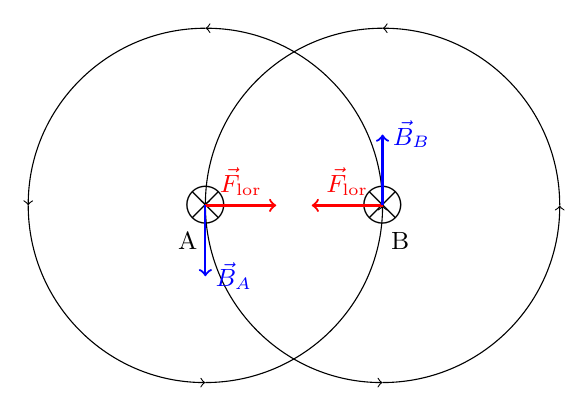
\begin{tikzpicture}[scale=4.5, every node/.style={font=\small}]
        % Drähte (Stromrichtung: in die Ebene), Abstand = 0.5
        \node at (0,0) {\huge\textbf{$\otimes$}};
        \node at (-0.05,-0.1) {A};

        \node at (0.5,0) {\huge\textbf{$\otimes$}};
        \node at (0.55,-0.1) {B};

        % Magnetfeldlinien von A (gegen Uhrzeigersinn), Radius = 0.5
        \draw[->] (0.5,0)   arc (0:90:0.5);
        \draw[->] (0,0.5)   arc (90:180:0.5);
        \draw[->] (-0.5,0)  arc (180:270:0.5);
        \draw[->] (0,-0.5)  arc (270:360:0.5);

        % Magnetfeldlinien von B (gegen Uhrzeigersinn), Radius = 0.5
        \draw[->] (1.0,0)       arc (0:90:0.5);
        \draw[->] (0.5,0.5)     arc (90:180:0.5);
        \draw[->] (0,0)         arc (180:270:0.5);
        \draw[->] (0.5,-0.5)    arc (270:360:0.5);

        % Lorentzkraft-Pfeile (rot)
        \draw[->, thick, red] (0,0.0)   -- (0.2,0.0)   node[midway, above] {$\vec{F}_{\mathrm{lor}}$};
        \draw[->, thick, red] (0.5,0.0) -- (0.3,0.0)   node[midway, above] {$\vec{F}_{\mathrm{lor}}$};

        % Magnetfeldrichtung (blau)
        \draw[->, thick, blue] (0,0.0)      -- (0,-0.2)     node[right] {$\vec{B}_A$};
        \draw[->, thick, blue] (0.5,0.0)    -- (0.5,0.2)    node[right] {$\vec{B}_B$};
    \end{tikzpicture}
    \caption{...}
    \label{fig:versuch2_parallele_leiter}
\end{figure}

\section{Versuche}

\begin{itemize}
    \item Superposition von Magnetfeldern
    \item Induktion zweier benachbarter Spulen
    \item Thomsonscher Ringversuch
\end{itemize}

\emph{Weitere Versuche hier einfügen.}
